\chapter{Test setup}

This section describes the used evaluation boards and bus transceivers for the test setup. Further, the test harness, realized by a breadboard is described. 
Figure \ref{fig:setup} shows a picture of the test setup, containing the breadboard (\gls{ECU}, \gls{THS}, \gls{MCU}, bus transceivers, switch, LED) and the Zedboard (\gls{FBU}). All components are supplied by the $3.3V$ power supply on the Zedboard.

\begin{figure}[h!]
    \centering
    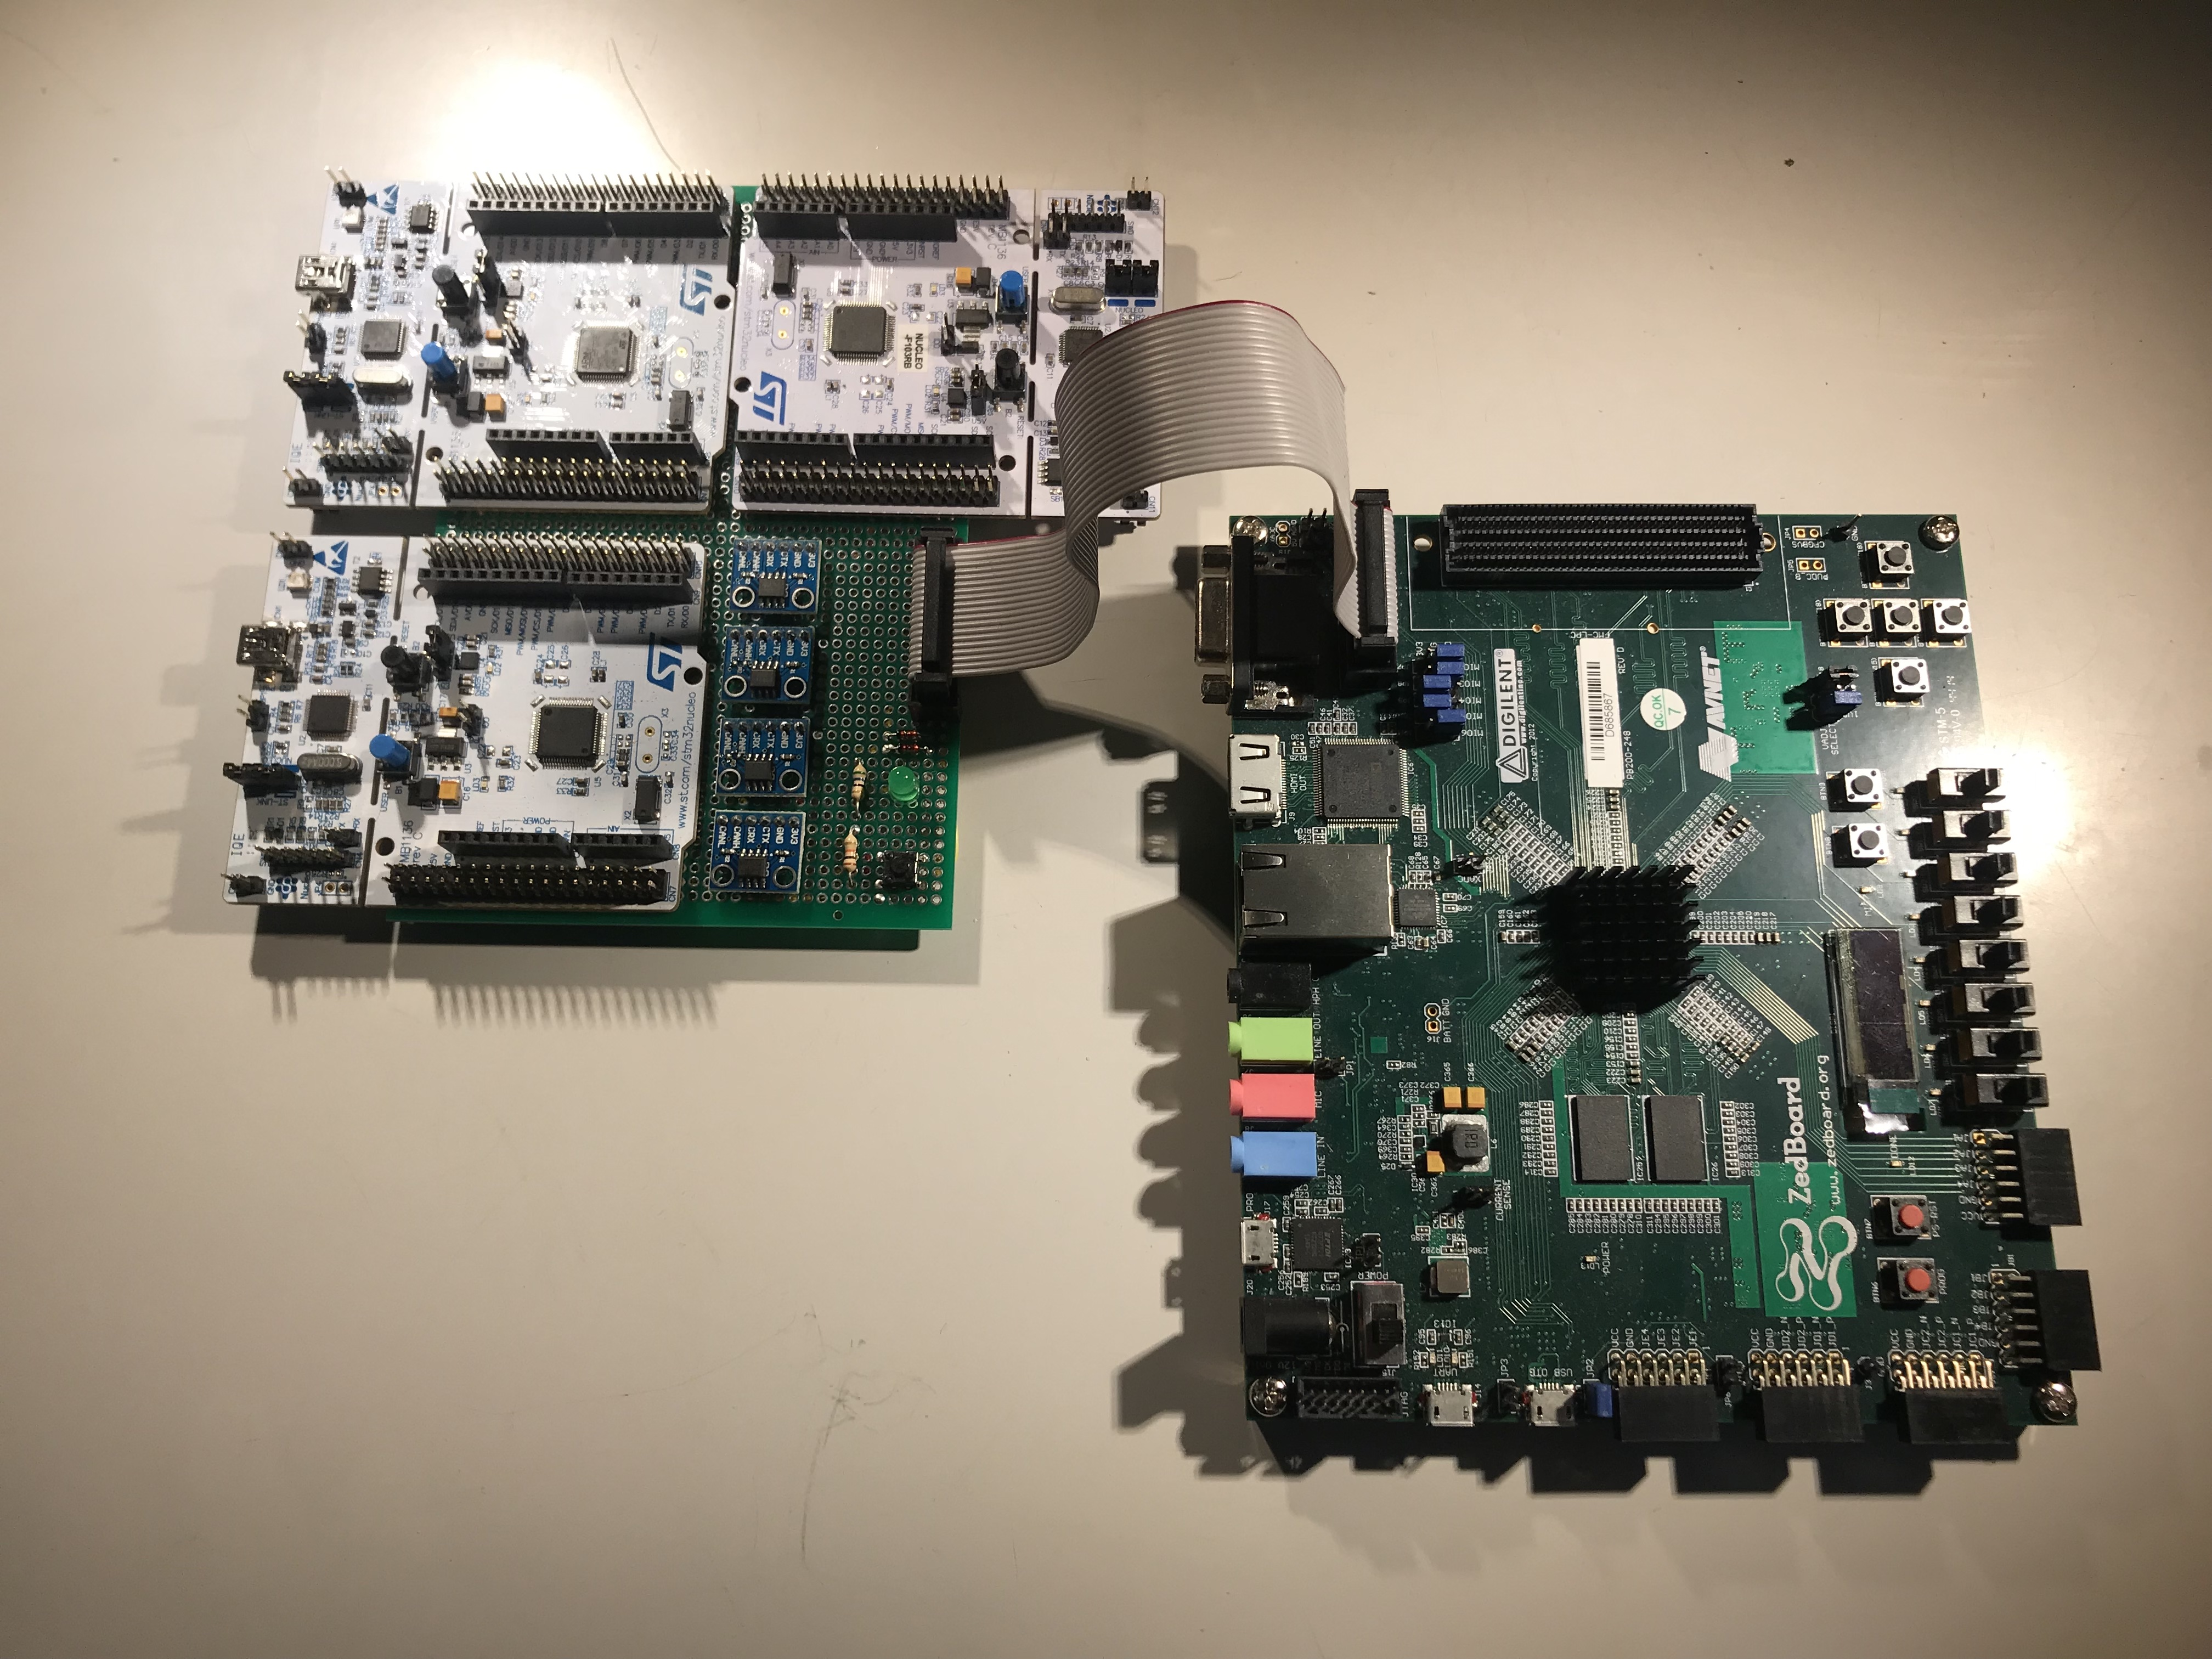
\includegraphics[width=\textwidth]{figures/hw_setup.jpg}
    \caption{Zedboard and STM32 hardware setup}\label{fig:setup}
\end{figure}

\section{Communication link}

In this approach CAN bus transceiver breakout boards, based on SN65HVD230 \cite{CANTransceiver} are used as physical layer below the communication protocol, described in section \ref{sec:protocol}. Figure \ref{fig:CANBus} shows a basic design for the physical bus setup.

\begin{figure}[h!]
    \centering
    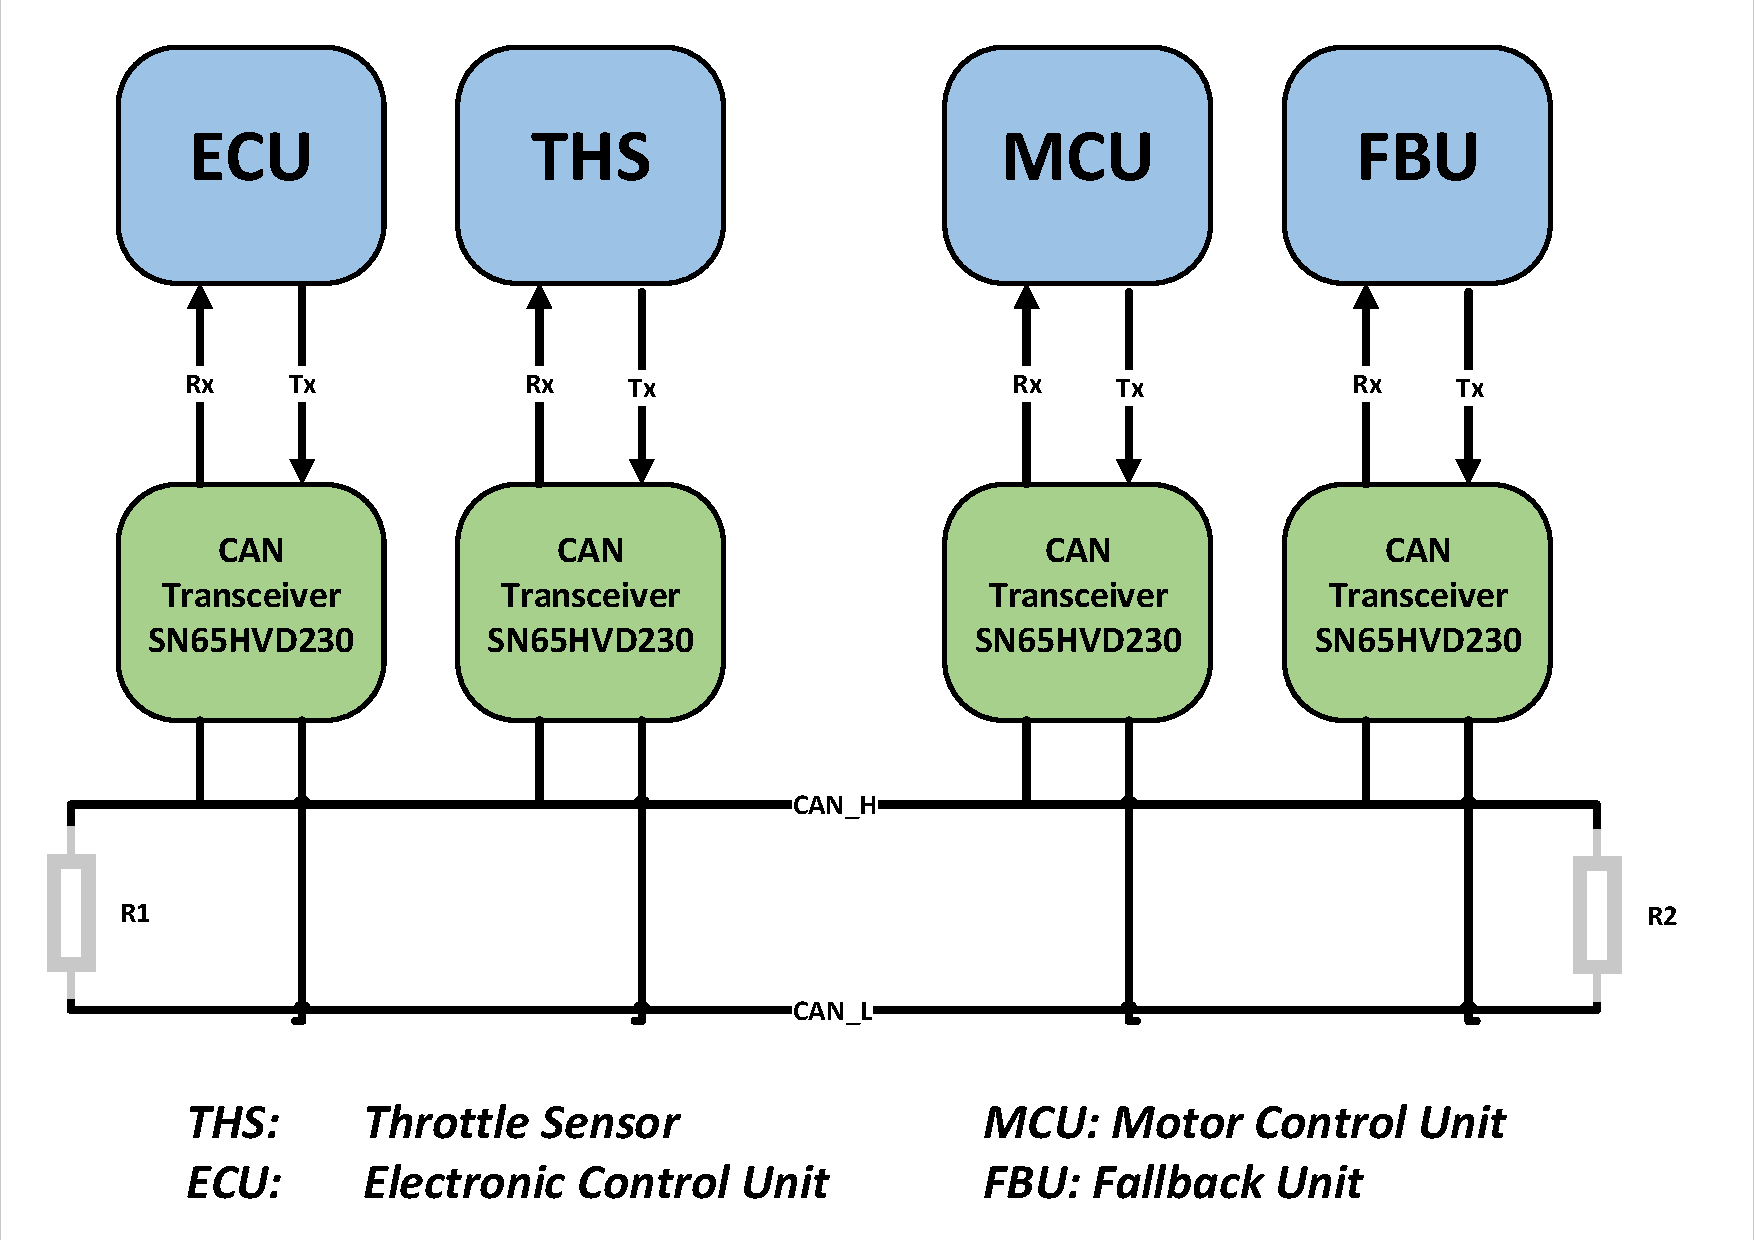
\includegraphics[width=\textwidth]{figures/CANBus4.pdf}
    \caption{CAN bus transceivers}\label{fig:CANBus}
\end{figure}

Each bus participant uses a CAN bus transceiver module to retrieve data from the (differential) bus through a UART interface.

\section{ECU, THS, MCU and FBU}

The \gls{ECU}, \gls{THS} and \gls{MCU} components are all implemented on Nucleo-64 Boards. The bus master (\gls{ECU}) is based on a Cortex M3 core \cite{STM32F103RB} available on a Nucleo-64 F103RB board \cite{NucleoBoard}, whereas the slaves (\gls{THS}, \gls{MCU}) are based on Cortex M0 cores \cite{STM32F072RB} on Nucleo-64 F072RB boards \cite{NucleoBoard}.

As sensor input a simple push button switch (simulating throttle position) is used, whereas as actuator output (simulating engine data) a LED is used.

The \gls{FBU} is implemented on a Zedboard \cite{ZedBoard}, which is a Zynq 7000 Evaluation Board.

\section{Connections}

To connect all Nucleo-64 boards, bus transceivers, push button and LED a breadboard was used. The ZedBoard and the breadboard are connected via a ribbon cable (Agile Mixed Signaling connector on the Zedboard). 
Since the \gls{FBU} must be able to use the sensor (push button) and actuator (LED), those peripherals are shared between \gls{THS} and \gls{FBU} (sensor) and between \gls{MCU} and \gls{FBU}.